\documentclass[spanish]{beamer}
\usepackage[utf8]{inputenc}
\usepackage[spanish]{babel}
\usetheme{Boadilla}
\usepackage{amsmath}
\usepackage{multicol}
\usepackage{textcomp}	
% Title, author, director, configurations
\title[MDIAE]{Diseño de una arquitectura tolerante a fallas basada en componentes COTS para vehículos satelitales de nueva generación}
\author{Arias Emmanuel}
\institute[UNLAM]{Universidad Nacional de la Matanza}
\date{\today}
\newcommand{\director}{Director: Ing. Gustavo Wiman}

% re-definition of the title page
\setbeamertemplate{title page}{
	\centering
	{\fontsize{18}{20}\selectfont
	\begin{beamercolorbox}[rounded=true,shadow=true,sep=8pt,center, dp=1cm]{title}
		\inserttitle \par
	\end{beamercolorbox}
    }
	\vfill
	\begin{columns}[T]
		\begin{column}{.23\textwidth}
			\centering
			
\includegraphics[scale=0.1]{images/logo-conae.png}
		\end{column}
		\begin{column}{.43\textwidth}
			\vbox to .3\textheight{%
				\centering
				Tesista: \insertauthor
				\vfill
				\director
				\vfill
				\vfill
				\usebeamerfont{institute}\insertinstitute \par
				\vfill
				\centering
				\insertdate\par
		    }
		\end{column}
		\begin{column}{.23\textwidth}
			\centering
			
\includegraphics[scale=0.2]{images/logo-invap.png}
			\vfill
			\centering
			
\includegraphics[scale=0.2]{images/logo-unlam.jpg}
		\end{column}
	\end{columns}
	
	\vfill
}

\begin{document}
\begin{frame}
	\titlepage
\end{frame}

% Table of content
\begin{frame}%[allowframebreaks]
    \frametitle{Agenda}
    \begin{multicols}{2}
	    \tableofcontents
	\end{multicols}
\end{frame}

\AtBeginSection[]
{
	\begin{frame}%[allowframebreaks]
		\frametitle{Agenda}
		\begin{multicols}{2}
		\tableofcontents[currentsection]
		\end{multicols}
	\end{frame}
}
\AtBeginSubsection[]
{
	\begin{frame}%[allowframebreaks]
		\frametitle{Agenda}
		\begin{multicols}{2}
			\tableofcontents[currentsubsection]	
		\end{multicols}
	\end{frame}
}


% Motivacion
\section{Motivación}
\begin{frame}
 \frametitle{Motivación}
	El desarrollo de proyecto satelitales conlleva costos de importante magnitud. Estos se pueden clasificar en 5 grandes grupo:
	\begin{itemize}
		\item Desarrollo
		\item Materiales
		\item Ensamblado, integración y test
		\item Lanzamiento
		\item Operaciones
	\end{itemize}
\end{frame}

%\subsection{Componentes COTS}
\begin{frame}
	\frametitle{Componentes COTS}
	\begin{itemize}
		\item Los componentes COTS suelen tener un costo de compra  de hasta 1000 veces menores que los componentes calificados para volar.
		\item Ayudaría a ahorrar millones de dólares de los proyectos satelitales. 
		\item La tecnología más avanzada de los COTS permite:
		\begin{itemize}
			\item Aumentar las prestaciones
			\item Implementar funciones que son imposibles con la tecnología actual
			\item Reducir tiempo de desarrollo
			\item Reducir volumen, masa y consumo de potencia.
		\end{itemize}
	\end{itemize}



	

	
	
\end{frame}

% Objetivos
\section{Objetivos}
\subsection{Objetivos del trabajo}
\begin{frame}
    \frametitle{Objetivo del trabajo}
    El objetivo de este trabajo es investigar y analizar arquitecturas de comunicación de los subsistemas de aviónica tolerante a fallas basada en componentes COTS para vehículos satelitales de nueva generación.
\end{frame}

\subsection{Objetivos específico}
\begin{frame}[allowframebreaks]
	\frametitle{Objetivo específico}
	\begin{enumerate}
		\item Realizar un estudio del estado de la cuestión sobre arquitecturas tolerantes a fallas para sistemas críticos.
		\item Investigar y analizar arquitecturas tolerantes a fallas que aseguren la confiabilidad del sistema y que sean aplicables en la industria satelital.
		\item Investigar y analizar protocolos de comunicación, para las capas superiores del modelo de OSI (modelo de interconexión de sistemas abiertos - ISO/IEC 7498-1), orientados a la tolerancia a fallas y confiabilidad de los sistemas. 
		\item Investigar una metodología para lograr una medición de la tolerancia a fallas en arquitecturas de aviónica.
		\item Desarrollar un estudio comparativo de arquitecturas tolerantes a fallas con el fin de obtener ventajas y desventajas de cada una de ellas.
		\item Diseñar modelos alternativos de arquitecturas tolerantes a fallas, que tengan un grado de confiabilidad tal, que permita la aplicación de componentes COTS.
		\item Evaluar la confiabilidad de los modelos de arquitecturas.
		\item Proponer el diseño de una nueva arquitectura tolerante a fallas, con un grado de confiabilidad suficiente para la aplicación de componentes COTS en avionicas de vehículos satelitales.
		\item Simular la arquitectura planteada para medir su grado de tolerancia a fallas y performance.
	\end{enumerate}
\end{frame}

\subsection{Preguntas de investigación}
\begin{frame}
	\frametitle{Preguntas de investigación}
	\begin{itemize}
		\item ¿Es posible la realización de un método de medición del grado de tolerancia a fallas de una arquitectura de aviónica?
		\item ¿Cuál es la estrategia más indicada de tolerancia a fallas que permita brindar un alto grado de confiabilidad en la utilización de componentes COTS en sistemas críticos?
		\item ¿Cuál es la arquitectura más indicada que permita desarrollar tolerancia a fallas en sistemas críticos basados en componentes COTS?
		\item ¿Es factible la utilización de componentes COTS en sistemas espaciales?
	\end{itemize}
\end{frame}

% que es la tolerancia a fallas
\section{¿Qué es la tolerancia a fallas?}
\begin{frame}
	\frametitle{¿Qué es la tolerancia a fallas?}
	\begin{columns}[T]
		\begin{column}{.5\textwidth}
			\centering
			Ariane 5 - 1996
			\vfill
			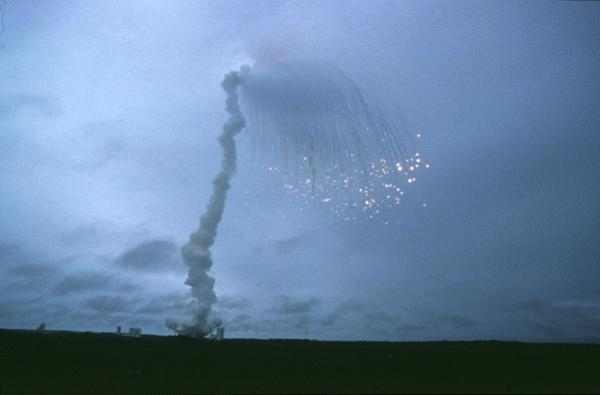
\includegraphics[scale=1]{images/ariane5.jpg}
		\end{column}
		\begin{column}{.5\textwidth}
			\begin{itemize}
				\item Approx. 30 seconds after lift-off the computer within the back-up inertial reference system ... became inoperative. This was caused by an internal variable ... exceeding a limit which existed in the software of this computer.
				\item Approx. 0.05 seconds later the active inertial reference system, identical to the back-up system in hardware and software, failed for the same reason.\footnote{Flight 501 Failure Report.Prof J. L.Lions}
			\end{itemize}
		\end{column}
	\end{columns}    
\end{frame}

\subsection{Atributos de la fiabilidad}
\begin{frame}
	\frametitle{Confiabilidad}
	Es la probabilidad de que un sistema continúe operando correctamente durante un intervalo de tiempo dado. 
	“Es la capacidad del sistema o componente de realizar sus funciones requeridos bajo las condiciones establecidas durante un período de tiempo específico” (IEEE)
	\LARGE
	$$
	R(t) = e^{-\lambda t }
	$$
\end{frame}

\begin{frame}
	\frametitle{Disponibilidad}
	Es la probabilidad de que el sistema esté operando correctamente en un determinado instante de tiempo. 
	\LARGE
	$$
	A(t) = 1/T \int_0^T{A(t) dt}
	$$
\end{frame}

\begin{frame}
	\frametitle{Seguridad}
	Se considera como una extensión de la confiabilidad. Se define como la probabilidad de que el sistema sea capaz de realizar sus funciones correctamente o continuar sus funciones en una manera a prueba de fallas. 
\end{frame}

\subsection{Falla, Error, Avería}
\begin{frame}[c]
	\begin{center}
		\LARGE
		\textbf{Falla \textrightarrow Error \textrightarrow Avería}\\
		\textit{Fault \textrightarrow Error \textrightarrow Failure}
	\end{center}
\end{frame}


% Marco teórico
%\section{Marco Teórico}
\subsection{Definiciones}
\begin{frame}
    \frametitle{Fallas != Error != Avería}
    \begin{itemize}
        \item \textbf{Avería:} ocurre cuando el servicio prestado por el sistema no coincide con las especificaciones del mismo.  Existe una consecuencia negativa en el sistema completo. (Failure)
        \item \textbf{Error:} es una parte del estado del sistema que es susceptible de provocar un avería en el sistema. Es una etapa intermedia entre falla y avería. (Error)
        \item \textbf{Falla:} también llamado “bug”. Es la hipótesis de un error. (Fault)
    \end{itemize}
\end{frame}

\begin{frame}
	\frametitle{Fallas de modo común vs fallas de causa común}
	\begin{itemize}
		\item \textbf{Fallas de modo común (CMF):}  es una falla que ocurre simultáneamente en dos o más componentes redundantes. CMF son causados por fenómenos que crean dependencias entre unidades redundadas.
		\item \textbf{Fallas de causa común (CCF):} se define como cualquier instancia donde múltiples elementos fallan debido a una causa común
	\end{itemize}
\end{frame}

\begin{frame}
	\frametitle{Fallas en el Software}
	Algunas de las fallas introducidas en el software:
	\begin{itemize}
		\item Especificaciones incorrecta de requerimientos
		\item Diseño incorrecto
		\item Errores de programación
	\end{itemize}
\end{frame}

\subsection{Medios y atributos de fiabilidad}
\begin{frame}
	\frametitle{Fiabilidad de sistemas}
	Algunas de las fallas introducidas en el software:
	La fiabilidad de un sistema es la capacidad del mismo de entregar a los usuarios un nivel deseado de servicio. 
	\vfill
	Es una medida de calidad que abarca los conceptos: confiabilidad, disponibilidad, y seguridad.
	\vfill
	Es un propiedad global que permite justificar la confianza de los servicios de un sistema 

\end{frame}

\begin{frame}
	\frametitle{Medios de fiabilidad}
	\begin{itemize}
		\item \textbf{Evitación de fallas:} técnicas de mejoramiento de la fiabilidad utilizadas durante el desarrollo de SW para reducir el número de fallas.  
        \item \textbf{Tolerancia a fallas:} se utiliza como una capa más de protección. FT es la capacidad del sistema a ejecutarse apropiadamente a pesar de la presencia de fallas. FT ocurre en tiempo de ejecución.
        \item \textbf{Eliminación de Fallas:} técnicas utilizadas para mejorar la fiabilidad empleadas durante el proceso de validación y verificación del sistema SW. Se eliminan la fallas que se detectan.
        \item \textbf{Predicción de Fallas:} se aplica mediante la realización de una evaluación del comportamiento del sistema con respecto a la ocurrencia, o la activación de una falla.
	\end{itemize}
\end{frame}

\subsection{Atributos de la fiabildad}
\begin{frame}
	\frametitle{Confiabilidad}
	Es la probabilidad de que un sistema continúe operando correctamente durante un intervalo de tiempo dado. 
	“Es la capacidad del sistema o componente de realizar sus funciones requeridos bajo las condiciones establecidas durante un período de tiempo específico” (IEEE)
	\LARGE
	$$
	R(t) = e^{-\lambda t }
	$$
\end{frame}

\begin{frame}
	\frametitle{Disponibilidad}
	Es la probabilidad de que el sistema esté operando correctamente en un determinado instante de tiempo. 
	\LARGE
	$$
	A(t) = 1/T \int_0^T{A(t) dt}
	$$
\end{frame}

\begin{frame}
	\frametitle{Seguridad}
	Se considera como una extensión de la confiabilidad. Se define como la probabilidad de que el sistema sea capaz de realizar sus funciones correctamente o continuar sus funciones en una manera a prueba de fallas. 
\end{frame}

\subsection{Medidas usadas en fiabilidad}
\begin{frame}
	\frametitle{Failure rate}
	Es el número esperado de fallas por unidad de tiempo. Generalmente, se encuentra a nivel de componente.
	\LARGE
	$$
	\lambda =  \sum_{i=1}^{n} \lambda_n
	$$	
\end{frame}

\begin{frame}
	\frametitle{Failure rate}
	\begin{columns}[T]
		\begin{column}{.5\textwidth}
			\centering
			Failure rate de HW vs tiempo
			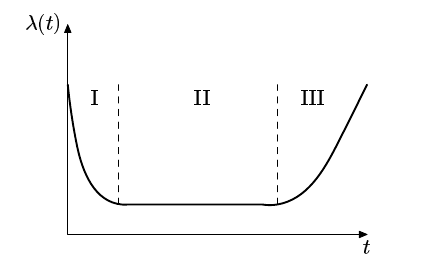
\includegraphics[scale=0.4]{images/bathtub_curve.png}
		\end{column}
		\begin{column}{.5\textwidth}
			\centering
			Failure rate de SW vs tiempo
			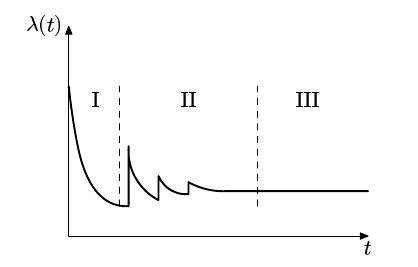
\includegraphics[scale=0.4]{images/Failure_rate_software.png}
		\end{column}
	\end{columns}
\end{frame}

\begin{frame}
	\frametitle{Failure rate}
    \textbf{Tiempo medio hasta la falla (MTTF):}
    $$ MTTF = \int_{0}^{\infty}{R(t) dt} $$
    \textbf{Tiempo medio de reparación (MTTR):}
    $$ MTTR = 1/\mu $$
\end{frame}

\subsection{Tolerancia a fallas}
\begin{frame}
	\frametitle{Tolerancia a fallas}
	\begin{columns}[T]
		\begin{column}{.5\textwidth}
			\centering
			Ariane 5 - 1996
			\vfill
			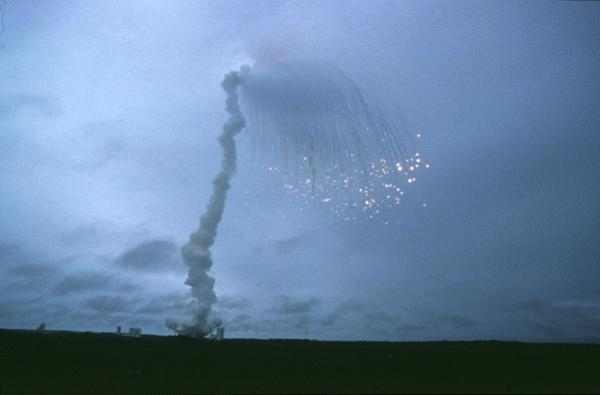
\includegraphics[scale=1]{images/ariane5.jpg}
		\end{column}
		\begin{column}{.5\textwidth}
			\centering
			Schiaparelli - 2016
			\vfill
			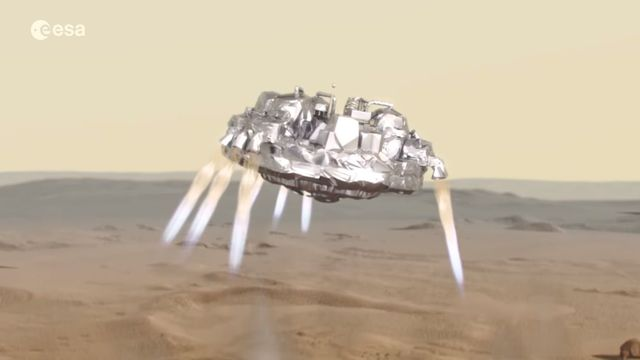
\includegraphics[scale=0.2]{images/mars.jpg}
		\end{column}
	\end{columns}    
\end{frame}

\begin{frame}
	\frametitle{Redundancia en el software}
	\begin{itemize}
		\item Técnicas single version
		\item Técnicas multi-version
		\item Técnicas de detección de fallas
		\item Técnicas de recuperación de fallas
	\end{itemize}
\end{frame}

% CAN bus
\section{Bus CAN}
\subsection{Definición}
\begin{frame}
	\frametitle{Bus CAN}
    \begin{columns}[T]
    	\begin{column}{.5\textwidth}
    		% \centering
    		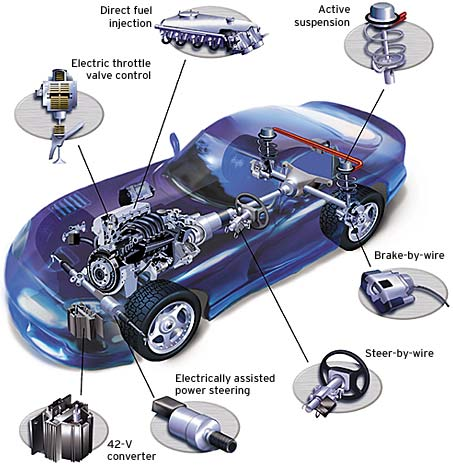
\includegraphics[scale=0.4]{images/ProtocoloCANAuto.png}
    	\end{column}
    	\begin{column}{.5\textwidth}
			\begin{itemize}
				\item Comenzó su desarrollo en 1983
				\item Estandarizado por la ISO (ISO 11898)
				\item Nació para ser usada en la industria automotriz
				\item Conectividad vía bus serial, a través de dos cables. 
				\item \textbf{Bajo costo}
			\end{itemize}
    	\end{column}
	\end{columns}
\end{frame}

\begin{frame}
	\frametitle{¿Por qué CAN Bus?}
	\vfill
	\begin{columns}[T]
		\begin{column}{.45\textwidth}
			\centering
			\vspace*{1cm}
			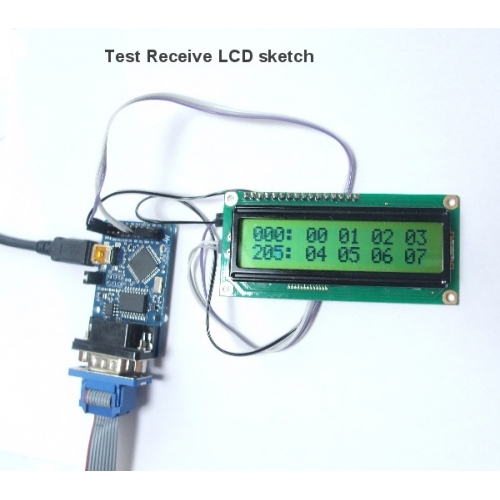
\includegraphics[scale=0.3]{images/bus_can.png}
		\end{column}
	    \begin{column}{.10\textwidth}
			\vspace*{3cm}
	    	\centering
	    	VS.
	    \end{column}
		\begin{column}{.45\textwidth}
			\centering
			\vspace*{2cm}
            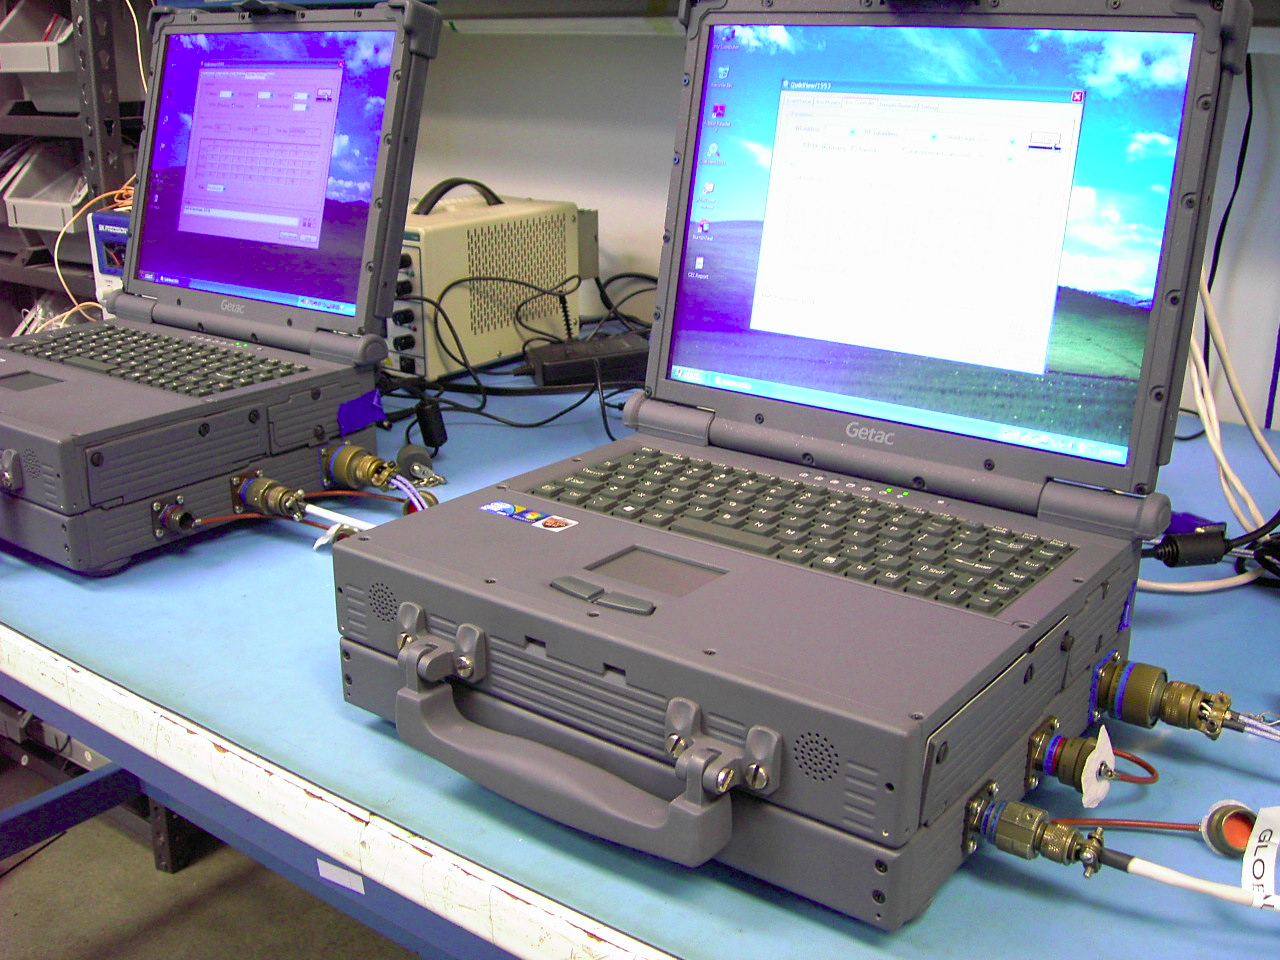
\includegraphics[scale=0.1]{images/1553.png}
		\end{column}
	\end{columns}
\end{frame}

\subsection{Protocolo CAN}
\begin{frame}
	\frametitle{Protocolo CAN}
	\begin{columns}[T]
		\begin{column}{.5\textwidth}
			\centering
			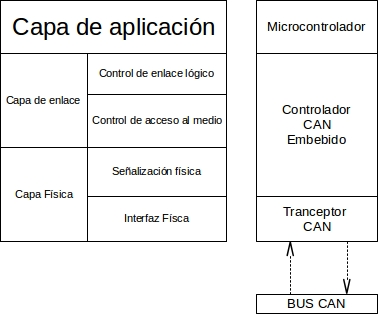
\includegraphics[scale=0.4]{images/ISO11898_Arquitectura_Standar.jpg}
		\end{column}
	    \begin{column}{.5\textwidth}
			\begin{table}[]
				\centering
				\begin{tabular}{c}
					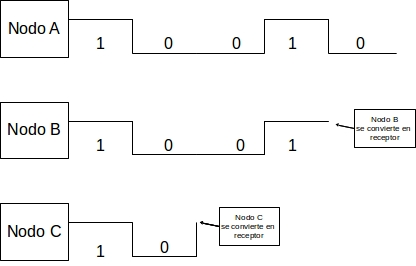
\includegraphics[scale=0.3]{images/CAN_BUS_Traffic.jpg} \\
					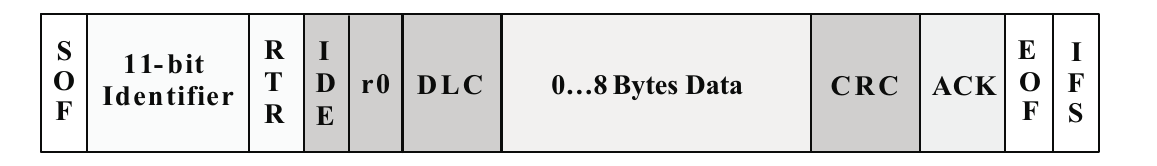
\includegraphics[scale=0.1]{images/StandarCAN.png} \\
					CAN Estándar \\ \hline
					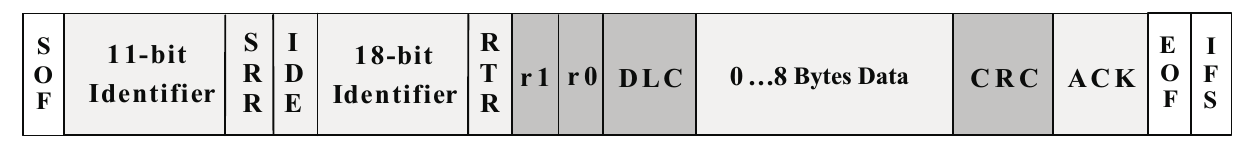
\includegraphics[scale=0.1]{images/ExtendedCAN.png} \\
					CAN Extendido \\
					\hline				
				\end{tabular}
			\end{table}
	    \end{column}
	\end{columns}
\end{frame}

% Estado del arte
%\section{Estado del arte}
\subsection{Árboles binarios}

\begin{frame}
    \frametitle{Árboles binarios}
    \begin{columns}[T]
    	\begin{column}{.5\textwidth}
    		% \centering
    		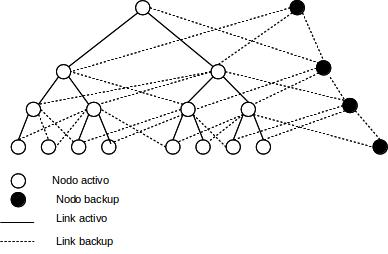
\includegraphics[scale=0.6]{images/binary_tree.jpg}
    	\end{column}
    	\begin{column}{.5\textwidth}
    		\begin{itemize}
    			\item Está compuesto por nodos y enlaces.
    			\item Está divididos en niveles. 
    			\item La FT de los árboles binarios vienen siendo estudiadas desde 1976.
    			\item Para lograr FT se las debe diseñar con un número mínimo de nodos de backup y link redundados. 
    		\end{itemize}
    	\end{column}
    \end{columns}
\end{frame}

\subsection{Redes Hypercube}
\begin{frame}
	\frametitle{Redes Hypercube}
	\begin{columns}[T]
		\begin{column}{.5\textwidth}
			% \centering
			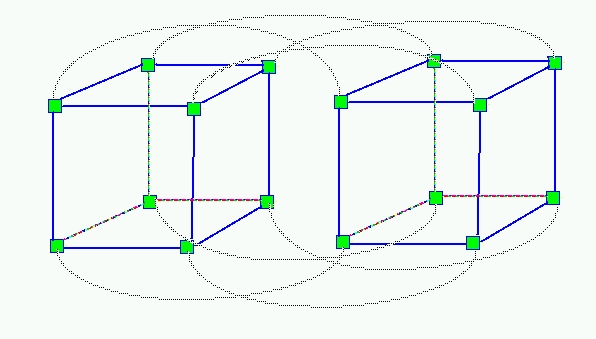
\includegraphics[scale=0.3]{images/cube.png}
		\end{column}
		\begin{column}{.5\textwidth}
			\begin{itemize}
				\item Tiene FT  de un componente. Si se produce una falla, no se transmite a todo el sistema. 
				\item Disponibilidad de enlaces entre cualquier par de nodos. 
				\item Existe una gran cantidad de enlaces. Esto aplicado en el ambiente espacial representa un problema. 
				
			\end{itemize}
		\end{column}
	\end{columns}
\end{frame}

\subsection{Redes distribuidas}
\begin{frame}
	\frametitle{Redes distribuidas}
	\begin{columns}[T]
		\begin{column}{.5\textwidth}
			% \centering
			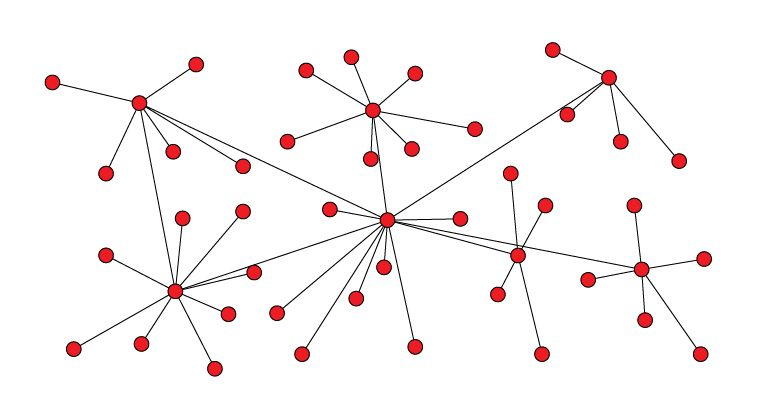
\includegraphics[scale=0.25]{images/distribuida.png}
		\end{column}
		\begin{column}{.5\textwidth}
			\begin{itemize}
				\item Red de nodos que se encuentran interconectados, intercambian información. 
				\item No existe un nodo central que gestione la red. 
				\item Una red distribuida es tolerante a fallas si puede formar subredes.
				\item Son necesarios el desarrollo y/o utilización de algoritmos de ruteo.
			\end{itemize}
		\end{column}
	\end{columns}
\end{frame}

\subsection{Redes TTEthernet en aviónica}
\begin{frame}
	\frametitle{Redes TTEthernet en aviónica}
	\begin{columns}[T]
		\begin{column}{.5\textwidth}
			% \centering
			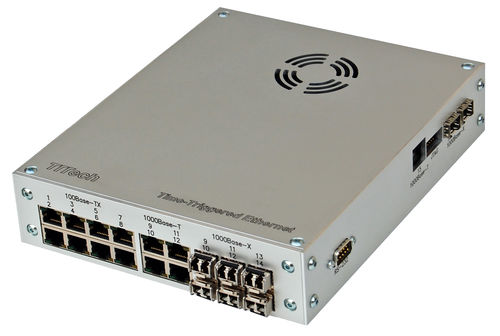
\includegraphics[scale=0.4]{images/ttethernet.png}
		\end{column}
		\begin{column}{.5\textwidth}
			\begin{itemize}
				\item TTEthernet es una tecnología basada en ethernet clásico. 
				\item Estandarizada como SAE AS6802.
				\item Transmite datos 100 veces más rápido que la que lo hacen las tecnologías tradicionales como el MIL-STD-1553.
				\item Fue utilizado en misiones como el Space Shuttle y la Estación Espacial Internacional (ISS).
			\end{itemize}
		\end{column}
	\end{columns}
\end{frame}

% Análisis de arquitectura tolerante a fallas
\section{Análisis de arquitectura tolerante a fallas}
\begin{frame}
	\begin{block}{Se supone una misión:}
		\begin{itemize}
			\item Misión de 15 años. 
			\item Sin payload.
			\item Formados por 6 subsistemas. 
			\item Como mínimo se tomarán 6 nodos en representación de los subsistemas.
			\item Cada nodo es una computadora con capacidad de procesamiento. 
			\item Cada nodo es un componente COTS.
		\end{itemize}
	\end{block}
\end{frame}

\begin{frame}
	Se concluye que las topologías que cumplen con los requerimientos y los objetivos de este trabajo de tesis son:
	\begin{itemize}
		\item Árboles binarios
		\item Redes distribuida
		\item Arquitectura hypercube
	\end{itemize}
\end{frame}

\begin{frame}
	\begin{columns}[T]
		\begin{column}{.5\textwidth}
			\begin{itemize}
				\item R(t) de árbol binario $$ R_sys = R^{2n+1} \prod_{k=0}^{n-1}{[(2^kc + 1) - 2^kcR]}$$
     		    \item R(t) de red hypercube $$ R_sys = 1 - |N(1-e^{\lambda t})|$$
     		    \item R(t) de red distribuida $$ R_sys = \sum_{i=0}^{k}{[(\prod_{v \exists S}{R(t)}) - (\prod_{\nexists S}{R(t)c})]}$$
			\end{itemize}
		\end{column}
		\begin{column}{.5\textwidth}
			% \centering
			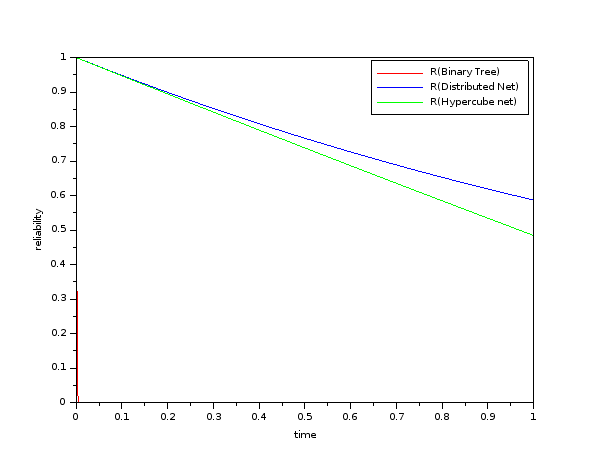
\includegraphics[scale=0.3]{images/comparative_reliablities.png}
		\end{column}
	\end{columns}
\end{frame}

% CANae
\section{CANae}
\subsection{Introducción}
\begin{frame}
	\frametitle{CANae}
	\begin{itemize}
		\item Surge de la necesidad de desarrollar un protocolo:
		\begin{itemize}
			\item Basado en el protocolo CAN
			\item Que actúe en las capas superiores del modelo de OSI
			\item Que permita la distribución de las tareas y el procesamiento llevado a cabo por los nodos
		\end{itemize}
		\item CANae se divide la capa de aplicaciones en dos:
		\begin{itemize}
			\item CANae Application Layer
			\item CANae High Application Layer
		\end{itemize}
	\end{itemize}
\end{frame}

\subsection{Capa de aplicación}
\begin{frame}
	\frametitle{Capa de Aplicación}
	\centering
	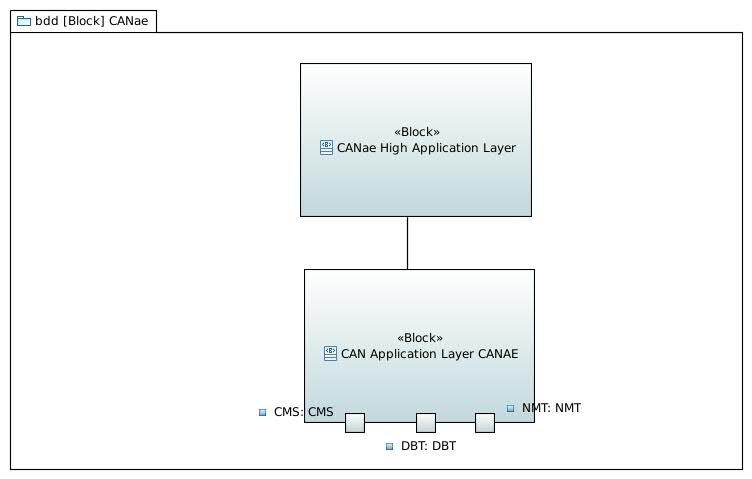
\includegraphics[scale=0.4]{images/CANAE.JPG}
\end{frame}

\subsection{CANae Application Layer}
\begin{frame}
	\frametitle{CANae Application Layer}
	\centering
	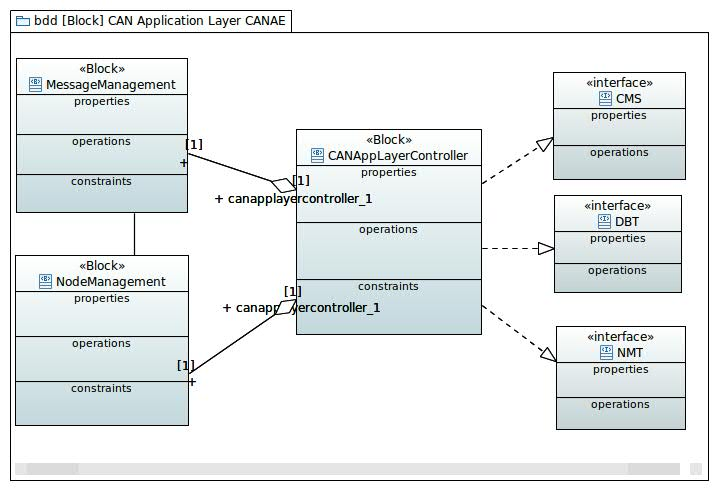
\includegraphics[scale=0.4]{images/CAN_Application_Layer_CANAE.jpg}
\end{frame}

% \subsection{CMS}
\begin{frame}
	\frametitle{CAN bassed Message Specification (CMS)}
	\centering
	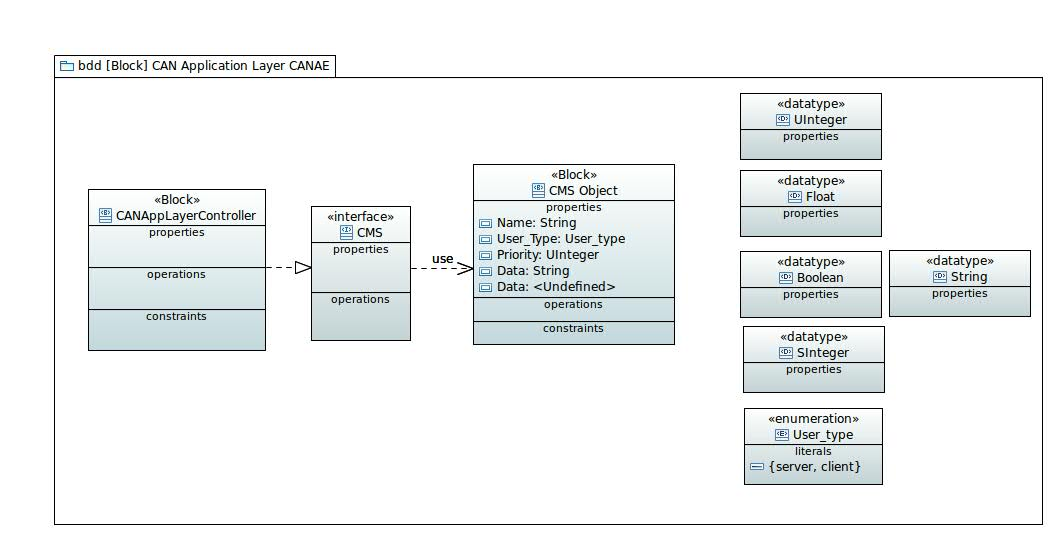
\includegraphics[scale=0.3]{images/CMS.JPG}
\end{frame}

% \subsection{NMT}
\begin{frame}
	\frametitle{Network Management (NMT)}
	\centering
	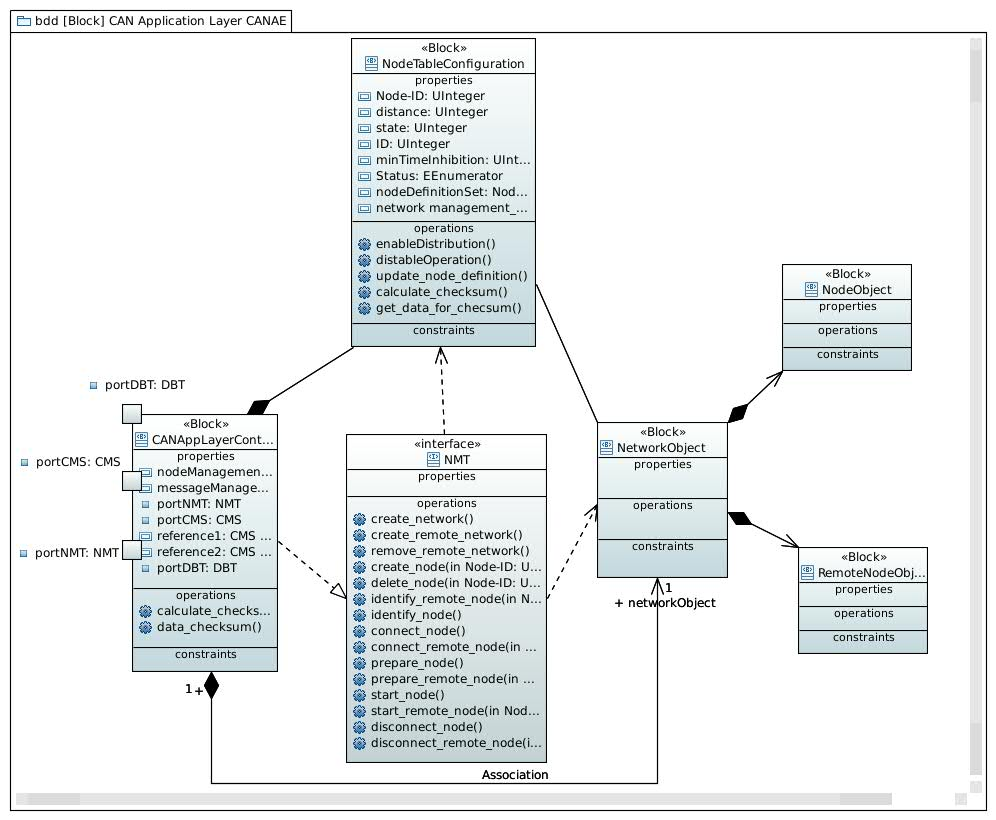
\includegraphics[scale=0.25]{images/NMT.JPG}
\end{frame}

% \subsection{DBT}
\begin{frame}
	\frametitle{Distributor (DBT)}
	\centering
	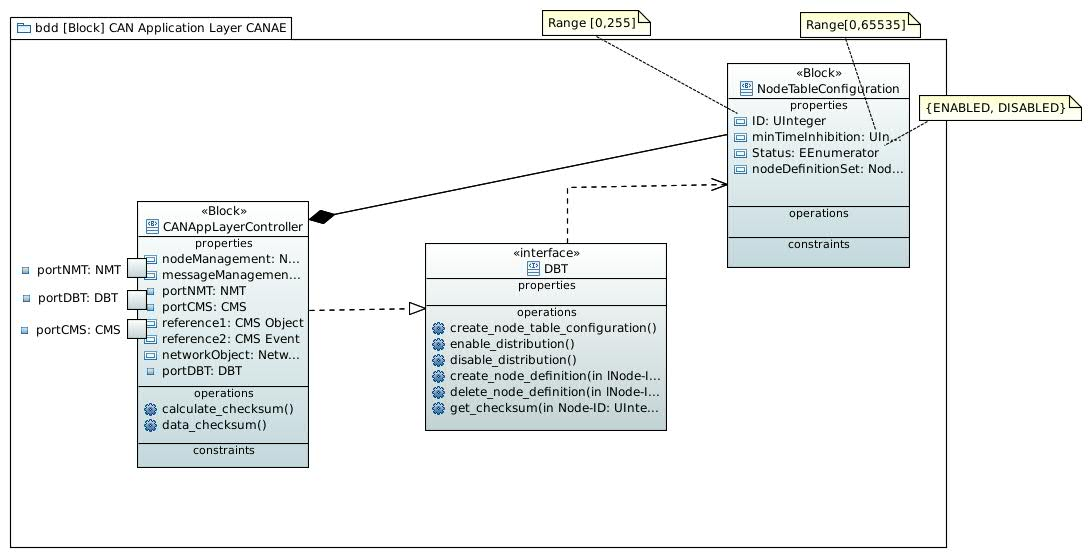
\includegraphics[scale=0.3]{images/DBT.JPG}
\end{frame}


\begin{frame}
	\frametitle{Gestor de mensajes}
	\centering
	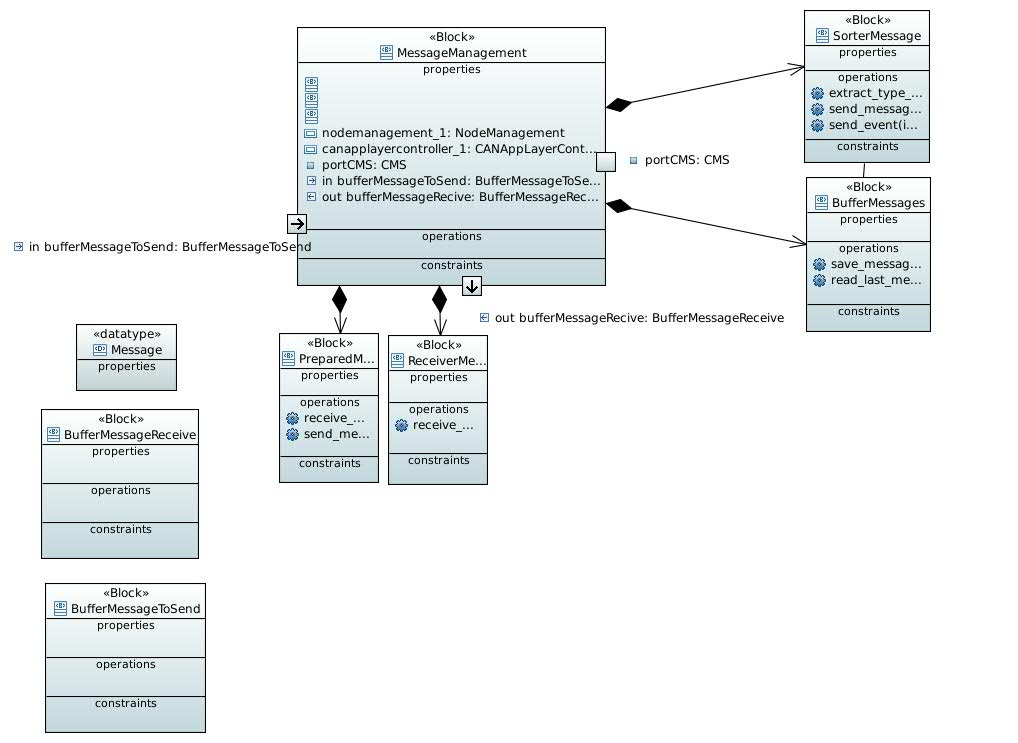
\includegraphics[scale=0.3]{images/MessageManagement.JPG}
\end{frame}

\begin{frame}
	\frametitle{Gestor de nodos}
	\centering
	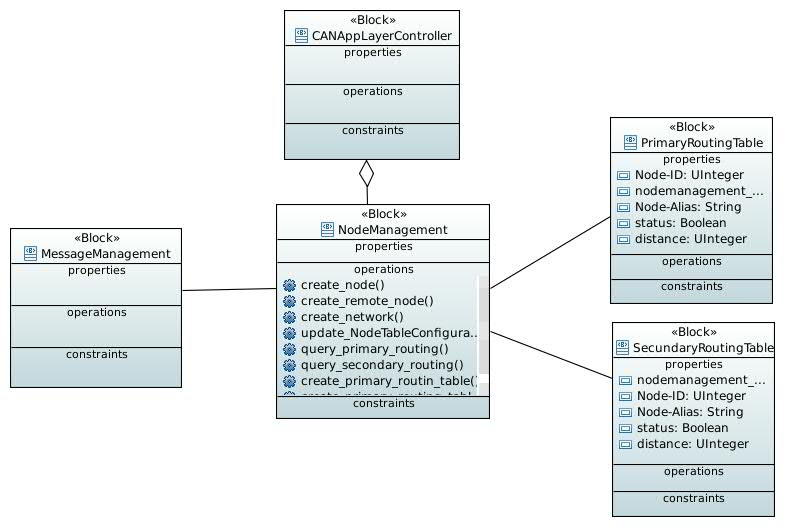
\includegraphics[scale=0.3]{images/NodeManagement.JPG}
\end{frame}

% \subsection{Formato de mensaje}
\begin{frame}
	\frametitle{Formato del mensaje}
	\centering
	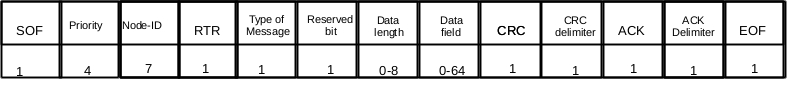
\includegraphics[scale=0.4]{images/Data_Frame.jpg}
\end{frame}

\subsection{High Application Layer CANae}
\begin{frame}
	\frametitle{High Application Layer CANae}
	\centering
	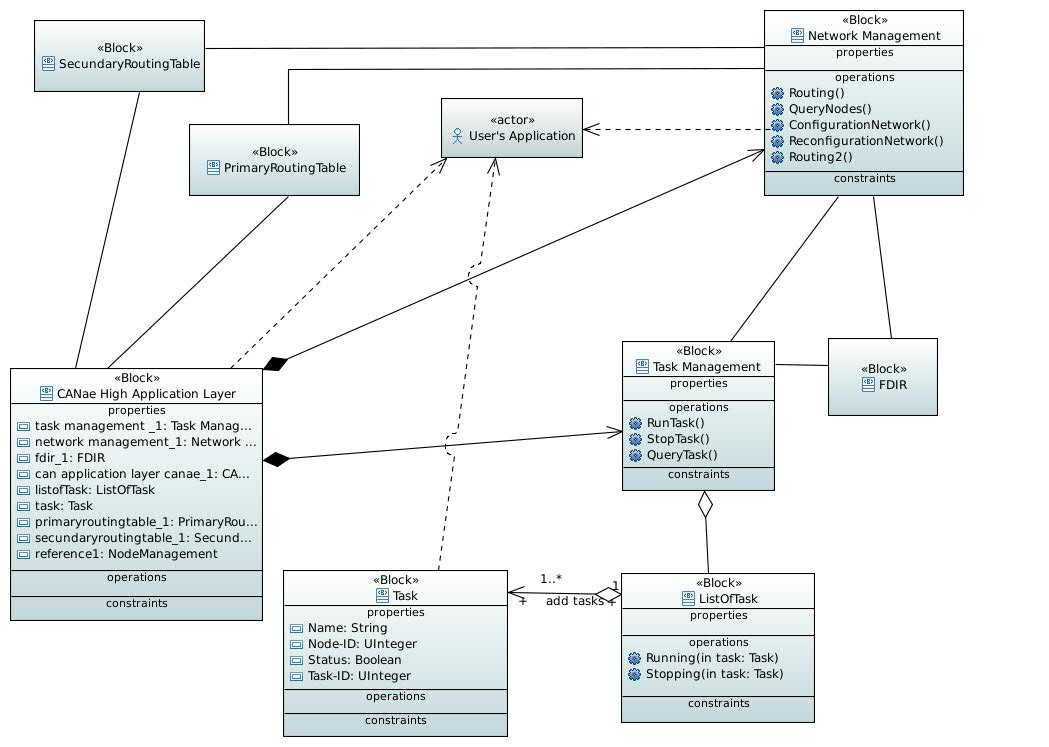
\includegraphics[scale=0.3]{images/CANae_High_App_Layer.JPG}
\end{frame}

% Arquitectura propuesta
\section{Arquitectura propuesta}
\begin{frame}
   \frametitle{Arquitectura propuesta}
   \begin{itemize}
   	\item Se centra en la comunicación de la aviónica de un vehículo espacial. 
   	\item Sus componentes primarios son de baja confiabilidad
   	\item Se utiliza el protocolo de comunicación CANae.
   	\item Se propone que la utilización de una filosofía distribuida
   \end{itemize}
\end{frame}

\begin{frame}[c]
		\centering
		\LARGE \textbf{Casos de usos}
\end{frame}

\begin{frame}
	% \centering
	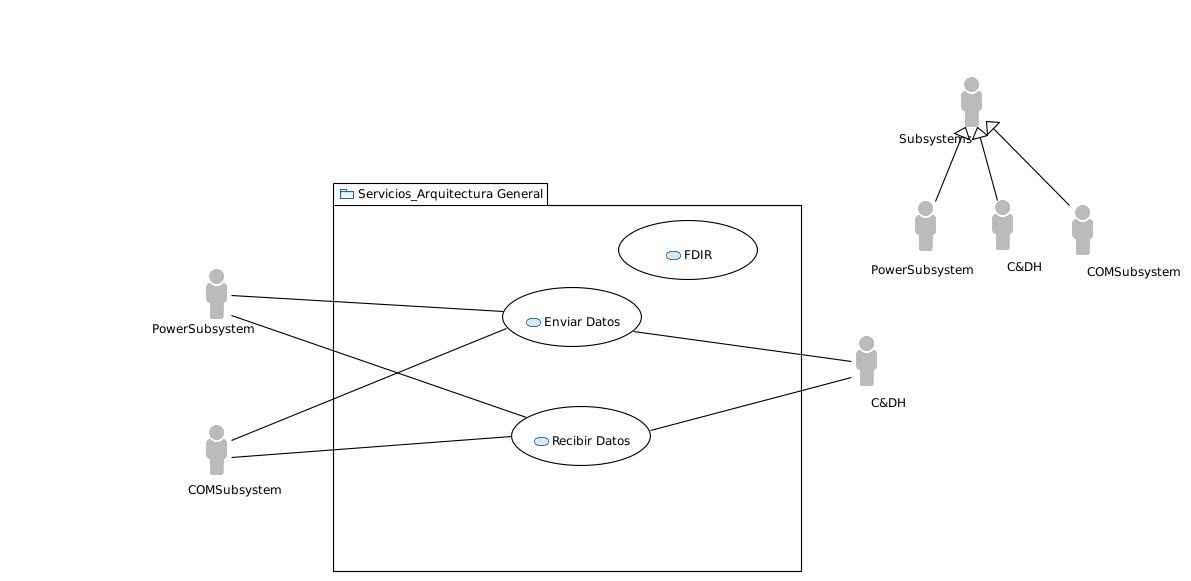
\includegraphics[scale=0.28]{images/Arq_General.JPG}
\end{frame}

\begin{frame}[c]
	\centering
	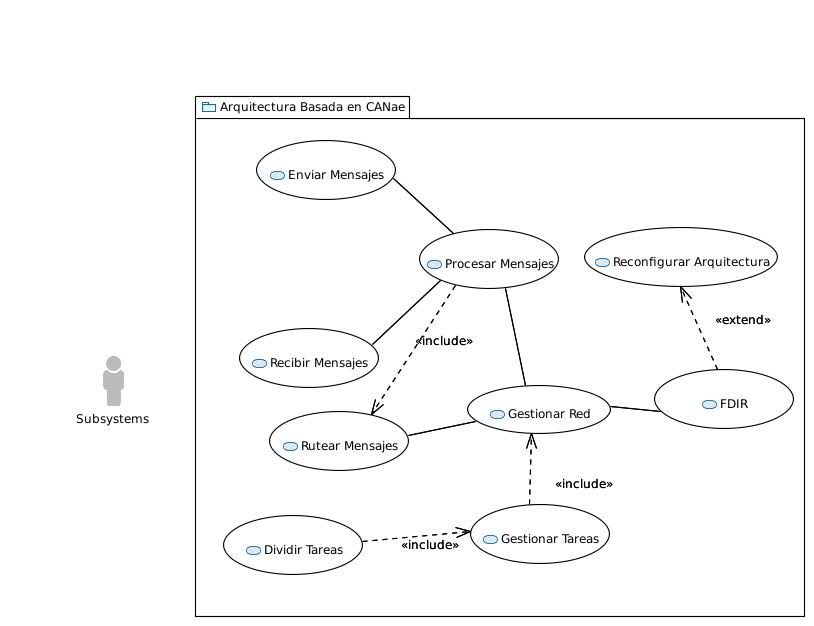
\includegraphics[scale=0.4]{images/Caso_de_Uso_Arquitectura.JPG}
\end{frame}
 
\begin{frame}[c]
	\centering
	\LARGE \textbf{Diseño estructural}
\end{frame}

\begin{frame}
	\frametitle{Diseño estructural}
	\begin{itemize}
		\item La arquitectura presentada rompe con el diseño tradicional de sistemas espaciales
		\item La arquitectura permite conectar una cantidad de N nodos (N < 128). Sus componentes son COTS. 
		\item La red a bajo nivel, deben trabajar bajo normas preestablecidas por algún protocolo preexistente. 
		\item Se aconseja el uso de CANOpen.
		\item Surge la necesidad de desarrollar un Bridge Tolerante a fallas. 
	\end{itemize}
\end{frame}

\begin{frame}[c]
	\centering
	\LARGE \textbf{Configuración de conexión}
\end{frame}

\begin{frame}[c]
	\centering
	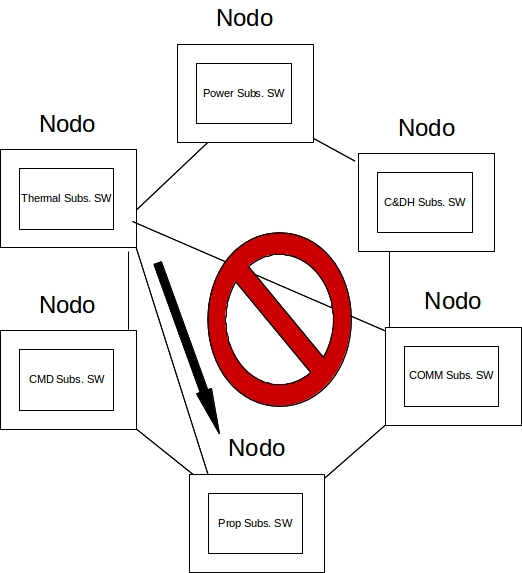
\includegraphics[scale=0.4]{images/Bridge1.jpg}
\end{frame}

\begin{frame}[c]
	\centering
	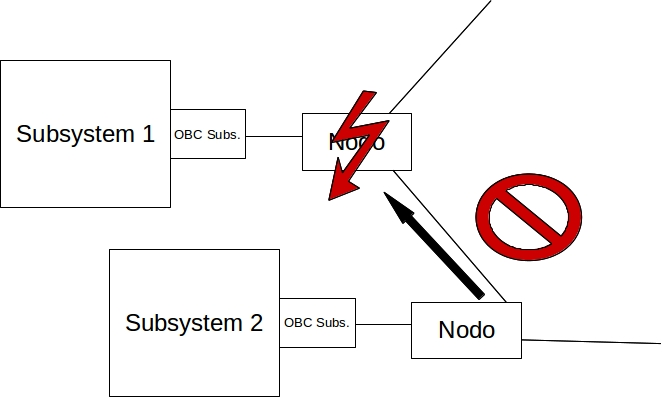
\includegraphics[scale=0.4]{images/Bridge2.jpg}
\end{frame}

\begin{frame}[c]
	\centering
	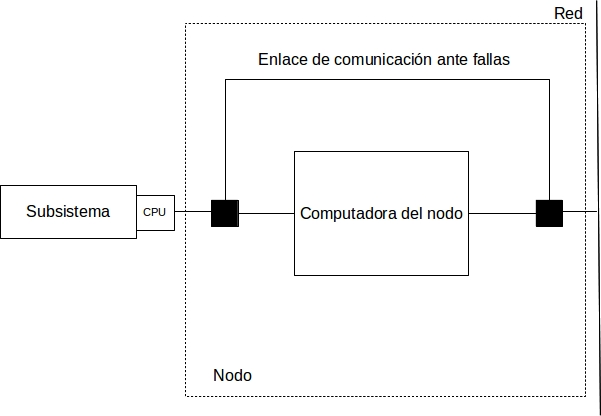
\includegraphics[scale=0.4]{images/com_nodo.jpg}
\end{frame}

\begin{frame}[c]
	\frametitle{Diseño estructural}
	\centering
	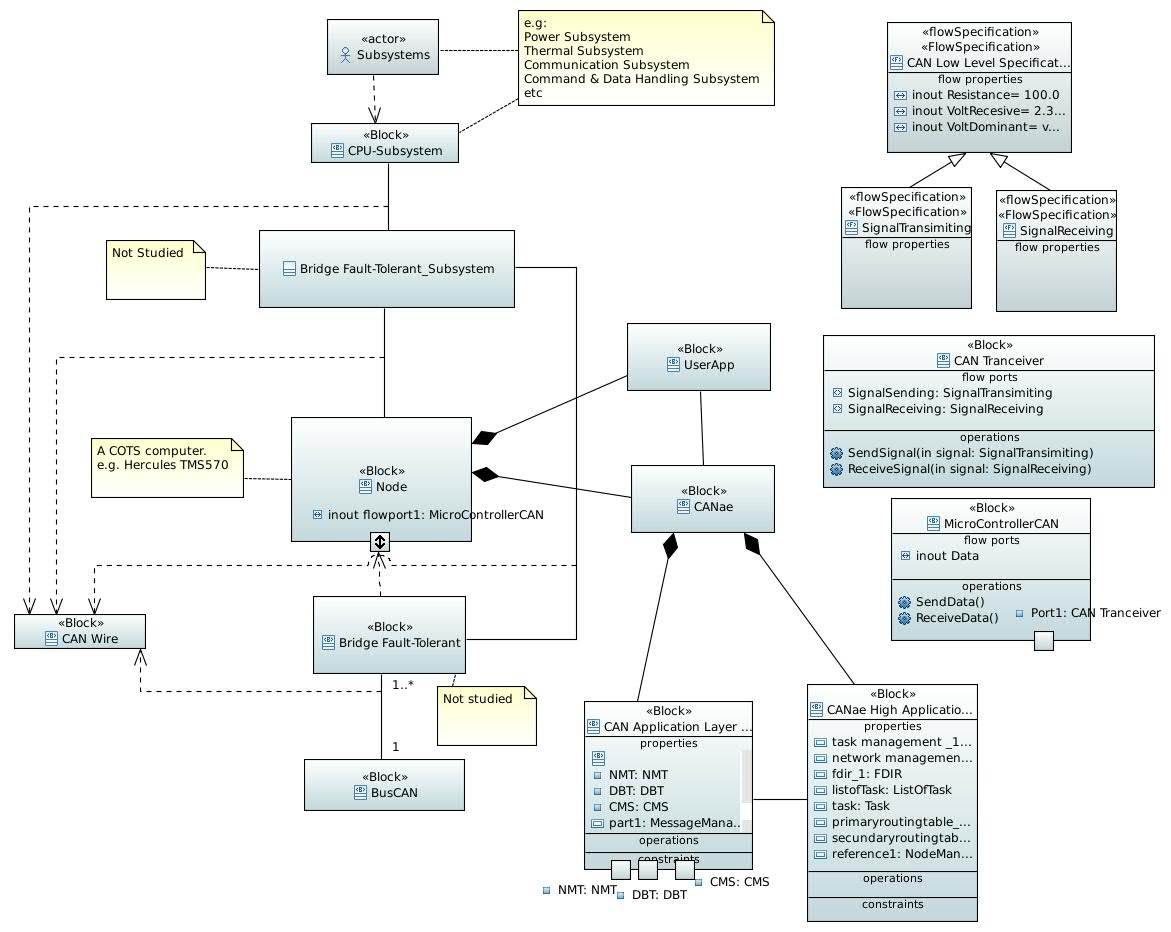
\includegraphics[scale=0.25]{images/ArqCompletaBlockDiagram.JPG}
\end{frame}

\begin{frame}[c]
	\frametitle{Nodo - Internal Block}
	\centering
	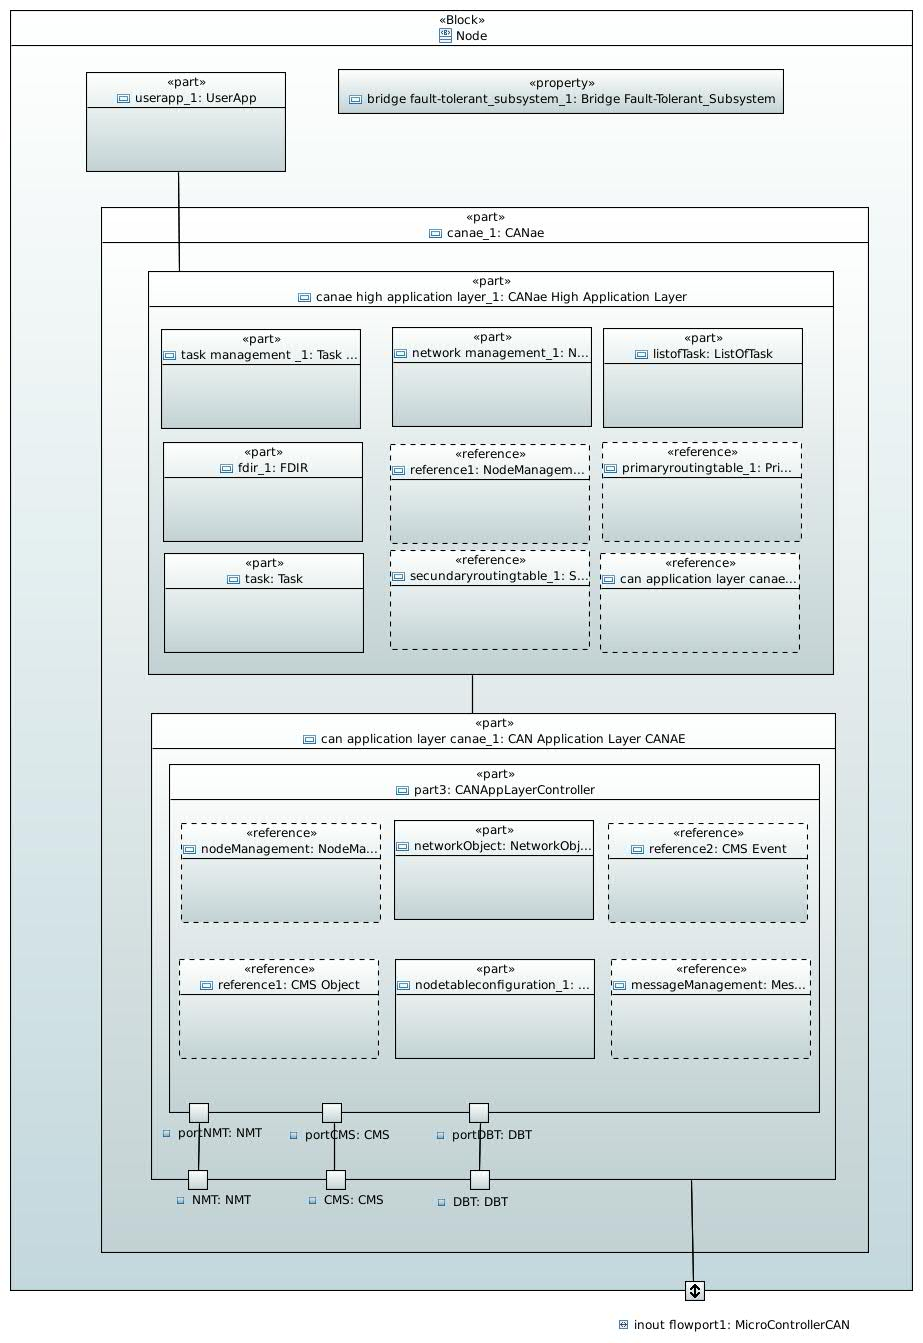
\includegraphics[scale=0.15]{images/NodeInternalDiagram.JPG}
\end{frame}

\begin{frame}[c]
	\centering
	\LARGE \textbf{Máquina de estado}
\end{frame}

\begin{frame}[c]
	\frametitle{Máquina de estado de la arquitectura completa}
	\centering
	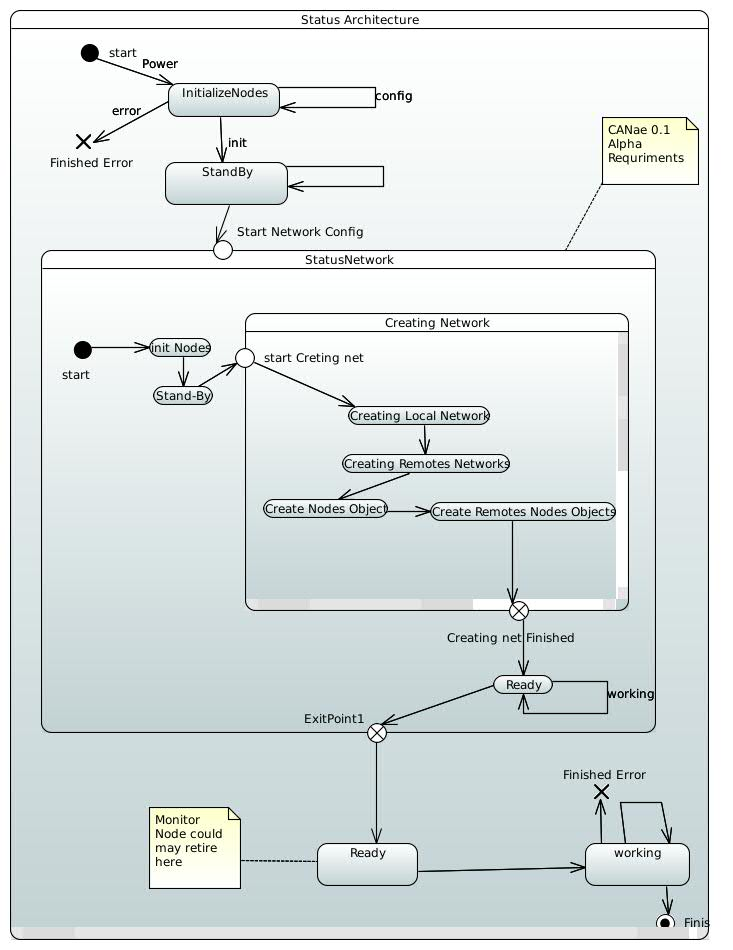
\includegraphics[scale=0.25]{images/StateMachineArqCompleta.JPG}
\end{frame}

\begin{frame}[c]
	\frametitle{Máquina de estado nodos}
	\centering
	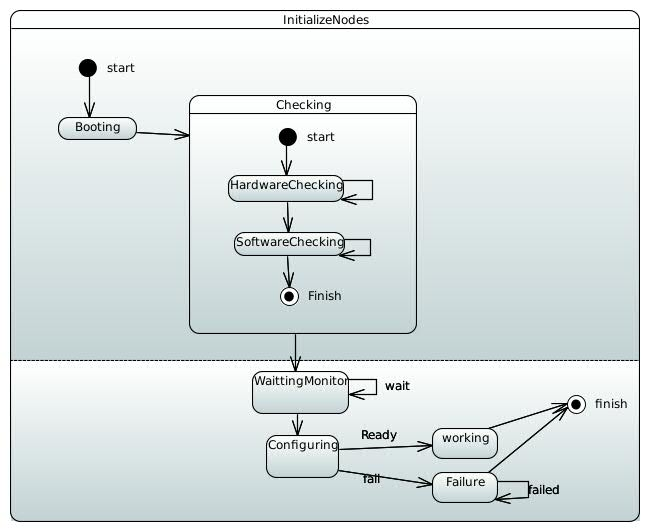
\includegraphics[scale=0.3]{images/InitializeNodes.JPG}
\end{frame}

\begin{frame}[c]
	\centering
	\LARGE \textbf{Diagramas de actividades}
\end{frame}

\begin{frame}[c]
	\frametitle{Inicio de Nodos}
	\centering
	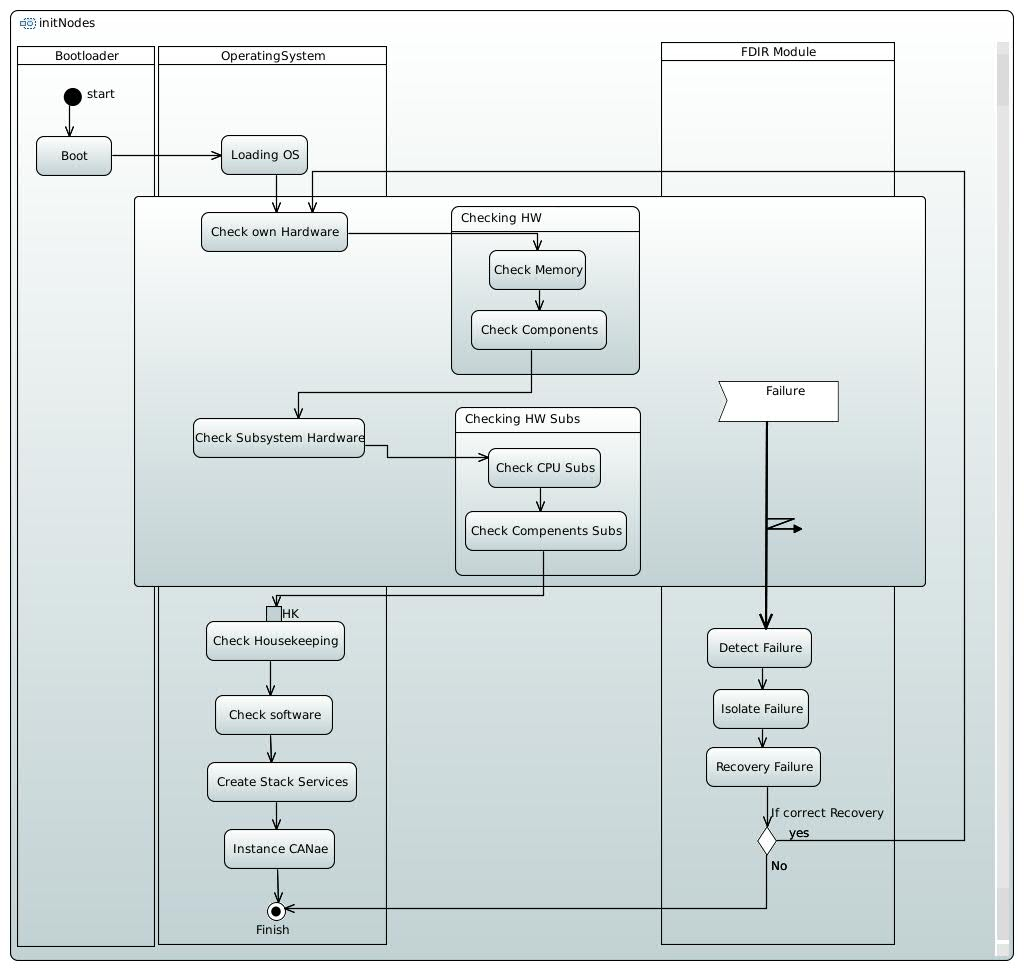
\includegraphics[scale=0.22]{images/initNodes.JPG}
\end{frame}

\begin{frame}[c]
	\frametitle{Nodo Monitor}
	\centering
	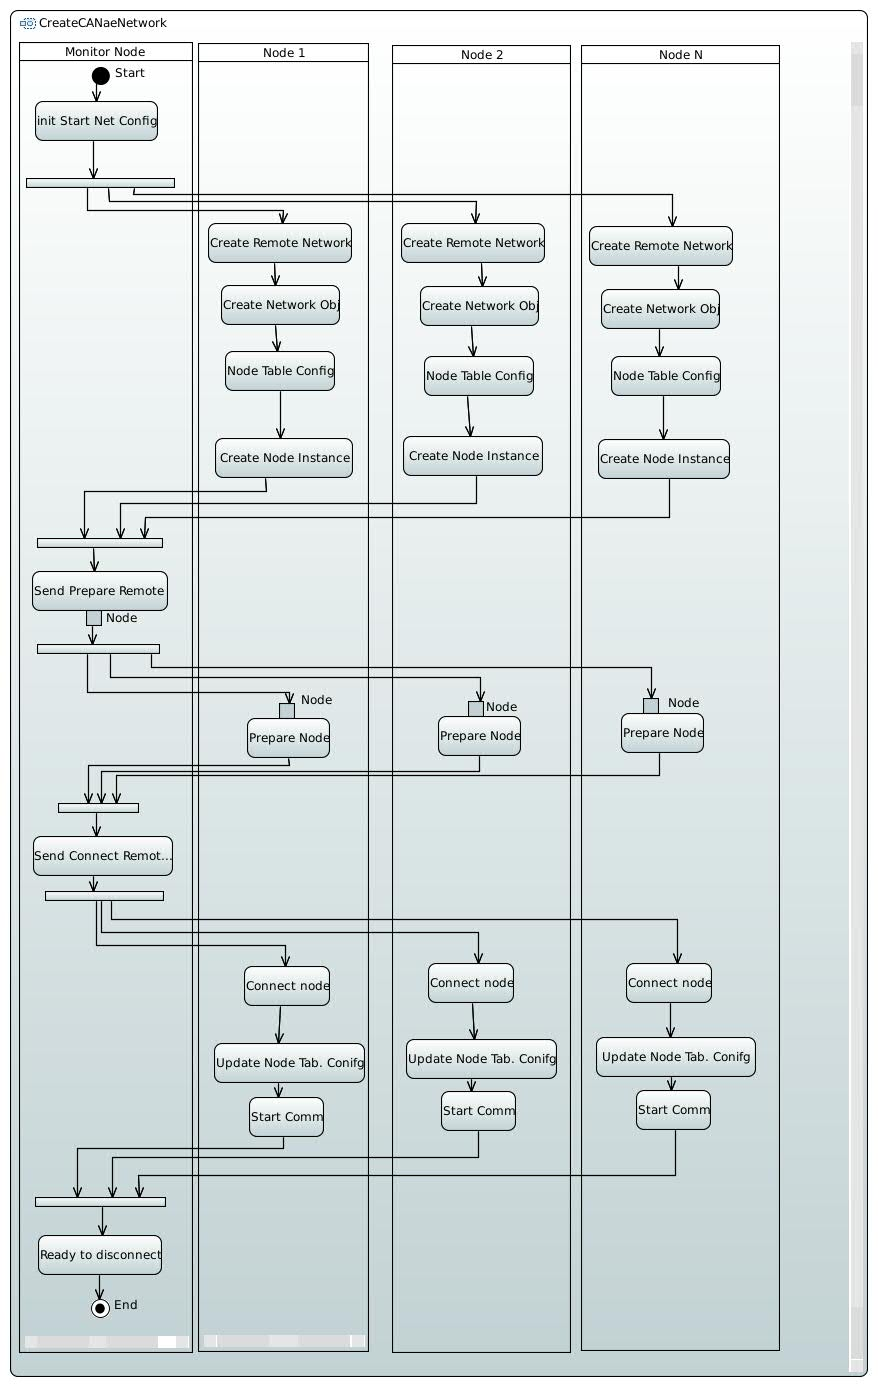
\includegraphics[scale=0.15]{images/NodeMonitor.JPG}
\end{frame}

% Conclusiones
\section{Conclusiones}
\begin{frame}
	\centering
	\LARGE \textbf{Conclusiones}
\end{frame}

\begin{frame}[c]
	\LARGE\centering
	\textbf{Muchas gracias por su atención}
\end{frame}

\appendix
\begin{frame}[noframenumbering, c]
	\LARGE
	\centering
	\textbf{Backup Slides}
\end{frame}
	
\end{document}
